
\documentclass[a4paper,12pt]{article}
\usepackage[a4paper, margin=2.4cm]{geometry}
\usepackage[utf8]{inputenc}
\usepackage{amsmath, amssymb} % Packages pour les maths
\usepackage[T1]{fontenc}
\usepackage{graphicx} 
\usepackage{caption}
\usepackage{setspace} % Espacement des lignes
\usepackage{tikz}





\begin{document}

\section{Modèle 1:}
\subsection{Bille remplie d'eau}
\textbf{Hypothèses}:
\begin{itemize}
    \item Terre assimilé à boule d'eau, de température \(T_{\text{Terre}}\) telle que \(T_{\text{Terre}}\)> \(T_{\text{vide}}\)
    \item  Sans atmosphère (dans le vide)
    \item  Sans puissance solaire reçue  
    \item \(C= C_{\text{eau}} \sim C_{\text{terre}}\) 
    \item $T(t=0) = T_i$ \ \ \
$T(t \to +\infty) = T_0$
   
\end{itemize}
$\rightarrow$ la terre perd de la température par rayonnement
\textbf{Equations :} 
\[   P= \sigma T^4 
\]

\[    C \, \frac{dT}{dt} = - \sigma T^4 \, dt \times S
\]

\[\frac{dT}{dt} = - \frac{4 \pi R_T^2 \sigma T^4}{C}\]  

\textbf{Solution:} 
\[
T(t) = \left( \frac{C}{C/T_i^3 + 12\pi R^2 \sigma t} \right)^{1/3} 
= \frac{T_i}{\left(1 + 3k T_i^3 t \right)^{1/3}}
\]
avec \(k=\frac{4\pi R_T^2 \sigma}{C}\)
et \(C=c_{\text{m eau}}\times m=4,60 \cdot 10^{27} J\cdot K^{-1}\)

\bigskip



\bigskip
\textbf{Modélisation:} 
    
    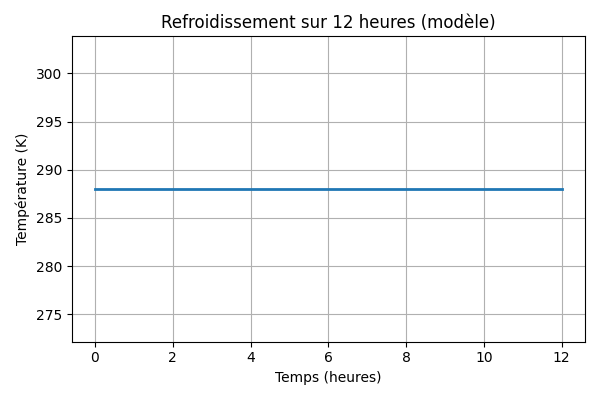
\includegraphics[width=0.8\linewidth]{../modele1/figures/modele1.png}
\\
\subsection{Coquille vide }
\textbf{Hypothèses}:
\begin{itemize}
    \item Terre assimilée à une coquille d'eau, d'épaisseur dr, avec du vide à l'intérieur
    
\end{itemize}
$\rightarrow$ il faut donc recalculer la capacitée thermique 


\begin{align*}
m &= \rho_{\text{eau}} \left( \frac{4}{3} \pi (R_T + dr)^3 - \frac{4}{3} \pi R_T^3 \right) \\
&\overset{DL}{\approx} \rho_{\text{eau}} \cdot 4\pi R_T^2 \cdot dr \\
\\
C &= c_{\text{eau}} \cdot \rho_{\text{eau}} \cdot 4\pi R_T^2 \cdot dr \\
&= 4{,}31 \cdot 10^{20} \ \text{J} \cdot \text{K}^{-1} \\
\\
k &= \frac{4\pi h }{c_{\text{eau}} \cdot \rho_{\text{eau}} \cdot 4\pi R^2 \cdot dr}
\end{align*}

    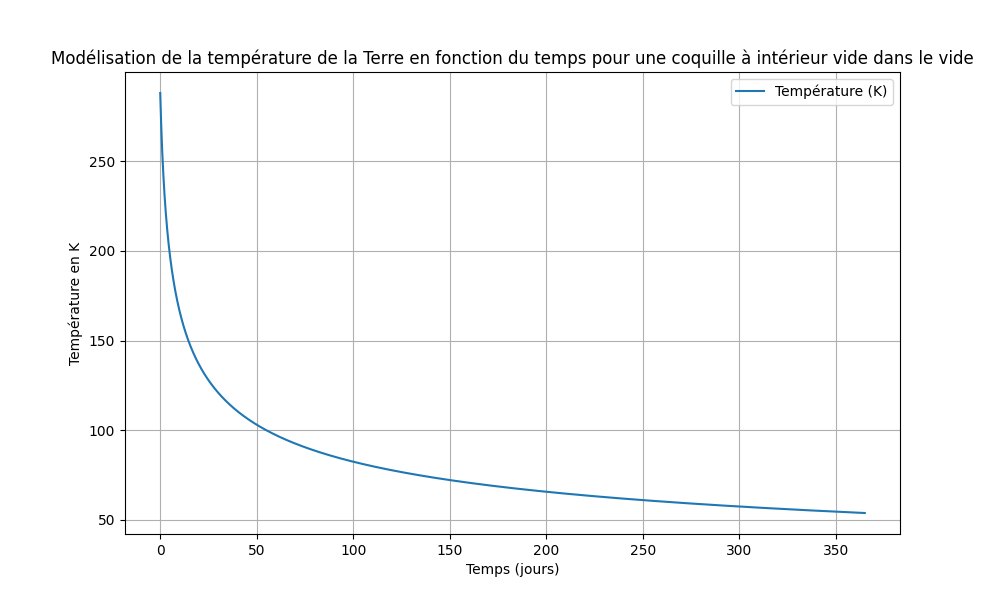
\includegraphics[width=0.8\linewidth]{../modele1/figures/modele1_coquille.png} 


\section{Modèle 2: Avec atmosphère}
\subsection{a. Boule d'eau avec atmosphère }
\textbf{Hypothèses}:
\begin{itemize}
    \item Terre assimilé à boule d'eau, de température \(T_{\text{Terre}}\) 
    \item  Athmosphère avec une température uniforme T 
    \item  Sans puissance solaire reçue  
    \item  ignorance de la convection  
    \item \(C_{\text{air}}\sim C_{\text{eau}}\) 
    \item $T(t=0) = T_i$ \ \ \
$T(t \to +\infty) = T_0$
   
\end{itemize}
\textbf{Équations de transfert thermique}

On introduira plus tard le \(P_{\text{th rayonnement}}\)

\begin{align*}
\delta Q &= c_{air}\, dT = -P_{\text{th,cond}} \cdot dt \\
\Rightarrow -\int \int \vec{j_{\text{th,cond}}}\, \vec{dS}\,dt = c_{air}\, dT \\
\Rightarrow -\int_{\theta=0}^\pi \int_{\phi=0}^{2\pi} h(T - T_0) \vec{e_{\text{r}}}\cdot r^2 \sin\theta\, d\theta\, d\varphi \vec{e_{\text{r}}}\, dt &=  c_{air}\, dT  \\
\Rightarrow -h(T - T_0) \cdot 4\pi\, dt &= c_{air}\, dT \\
\Rightarrow -T + T_0 = \frac{c}{h 4\pi} \frac{dT}{dt} \Rightarrow \frac{dT}{dt} &= -\frac{4\pi h}{c}(T - T_0)
\end{align*}

\vspace{0.5cm}

\textbf{Solution:} 
$T(t) = T_0 + (T_i - T_0)e^{-kt}$ \quad avec $k = \frac{4\pi h}{c}$

\subsection{b. Coquille assimilée à de l'eau avec atmosphère }
schéma Melvin

\section{Modèle 3: Avec intérieur de la coquille non vide }
\textbf{Hypothèses}:
\begin{itemize}
    \item Terre assimilée à une coquille d'eau avec intérieur non vide 
    \item  conduction entre entre centre de la terre et croûte 
    \item  conduction entre croûte et air 
    \item  rayonnement de la croûte
    
    
    
\end{itemize}


\[
(-P_{\mathrm{th,cond}} - P_{\mathrm{th,ray}} + P_r)\,dt = C\,dT.
\]

\[
-\,h\bigl[T(r+dr)-T_0\bigr]\;4\pi
\;-\;4\pi\,(r+dr)^2\,\sigma\,T^4(r+dr)
\;-\;4\pi\,r^2\,\lambda\,\frac{\partial T}{\partial r}(r)
\;=\;C\,\frac{dT}{dt}.
\]

\medskip

Or au \(1^{er}\) ordre en \(dr\), \(r+dr\approx r\) :

\[
-4\pi\,h\bigl(T(r)-T_0\bigr)
\;-\;4\pi\,r^2\,\sigma\,T(r)^4
\;-\;4\pi\,r^2\,\lambda\,\frac{\partial T}{\partial r}(r)
\;=\;C\,\frac{dT}{dt}.
\]

\medskip

Avec
\[
P_{r}
= \iint\vec j_{\mathrm{thr}}\cdot d\vec S
= \iint -\lambda\,\nabla T\cdot d\vec S
= -\lambda
  \int_{0}^{\pi}\!\!\int_{0}^{2\pi}
    \frac{\partial T}{\partial r}\,\vec e_{r}\,
    r^2\sin\theta\;d\theta\,d\varphi\;\vec e_{r}
= -\lambda\,4\pi\,r^2\,\frac{\partial T}{\partial r}.
\]


 
\vspace{1cm}


\end{document}
